\subsection{Funktionen der App}
        In den folgenden Abschnitten werden die Funktionen der App dargestellt 
        und erklärt. Im Kontext der jeweiligen Funktion werden beispielhaft einzelne 
        Methodenimplementationen herausgenommen,erklärt  und erörtert.
        Außerdem werden Design-Entscheidungen skizziert um die Nutzer-Erfahrung zu 
        visualisieren.   
        
\subsubsection{Rollen und Registrierung}
        Wie bereits in der Zielsetzung dargestellt, soll es ein Berechtigungssystem 
        für die App geben. Unterteilt wird dieses in die Rollen \glqq Sanitäter/-in\grqq{} 
        und \glqq Alarmierende/-n\grqq{}. Alarmierende sollen nur in der Lage sein einen Alarm 
        auszulösen und die Alarmierenden-News, sowie die Notfallnummern einzusehen.
        Anders als die Alarmierenden sollen Sanitäter/-innen auch in der Lage sein 
        einen Alarm zu empfangen und andere Sanitäter/-innen zu vertreten oder sich 
        aus dem Dienstplan auszutragen. Um dies umzusetzen muss bereits bei der 
        Registrierung darauf geachtet werden, wer welche Rolle zugewiesen bekommt.
        Im Folgenden erkläre ich jetzt, zunächst beispielhaft, wie die Registrierung 
        für eine/-n Sanitäter/-in abläuft und erläutere im Anschluss, welche Unterschiede es 
        bei der Registrierung für Alarmierende gibt.
        \newline\\
        Zunächst muss der/die Nutzer/-in den ihr/ihm zugehörigen Sanitätsdienst 
        auswählen. Um diesen auszuwählen muss der / die Nutzer/-in auf 
        den gewünschten Sanitätsdienst klicken. Wenn dieser nicht direkt erscheint, 
        ist es außerdem möglich diesen mit der im View (Mit dem Wort View beschreibe ich die unterschiedlichen
        Benutzeroberflächen, welche ich implementiert habe) oben angelegten Suchleiste herauszusuchen.  
        Im Anschluss muss der/die Nutzer/-in auf den \glqq Weiter\grqq{}-Button klicken um sich
        darauf folgend anzumelden oder zu registrieren. 
        Zusätzlich verdeutlicht der Button durch unterschiedliche Farbanzeige, ob ein Anklicken erfolgen kann oder nicht.
        Erscheint der Button grau, ist ein Anklicken nicht möglich und macht deutlich, dass bisher kein Sanitätsdienst 
        ausgewählt wurde. Erscheint der Button in der Farbe grün, besteht die Möglichkeit den Button anzuklicken, da bereits
        ein Sanitätsdienst ausgewählt wurde.
        \\In Abbildung 1 ist der View zu sehen, 
        in welchem der Sanitätsdienst ausgewählt wird.
        
        %\begin{figure}[H]
        %    \begin{center}
        %       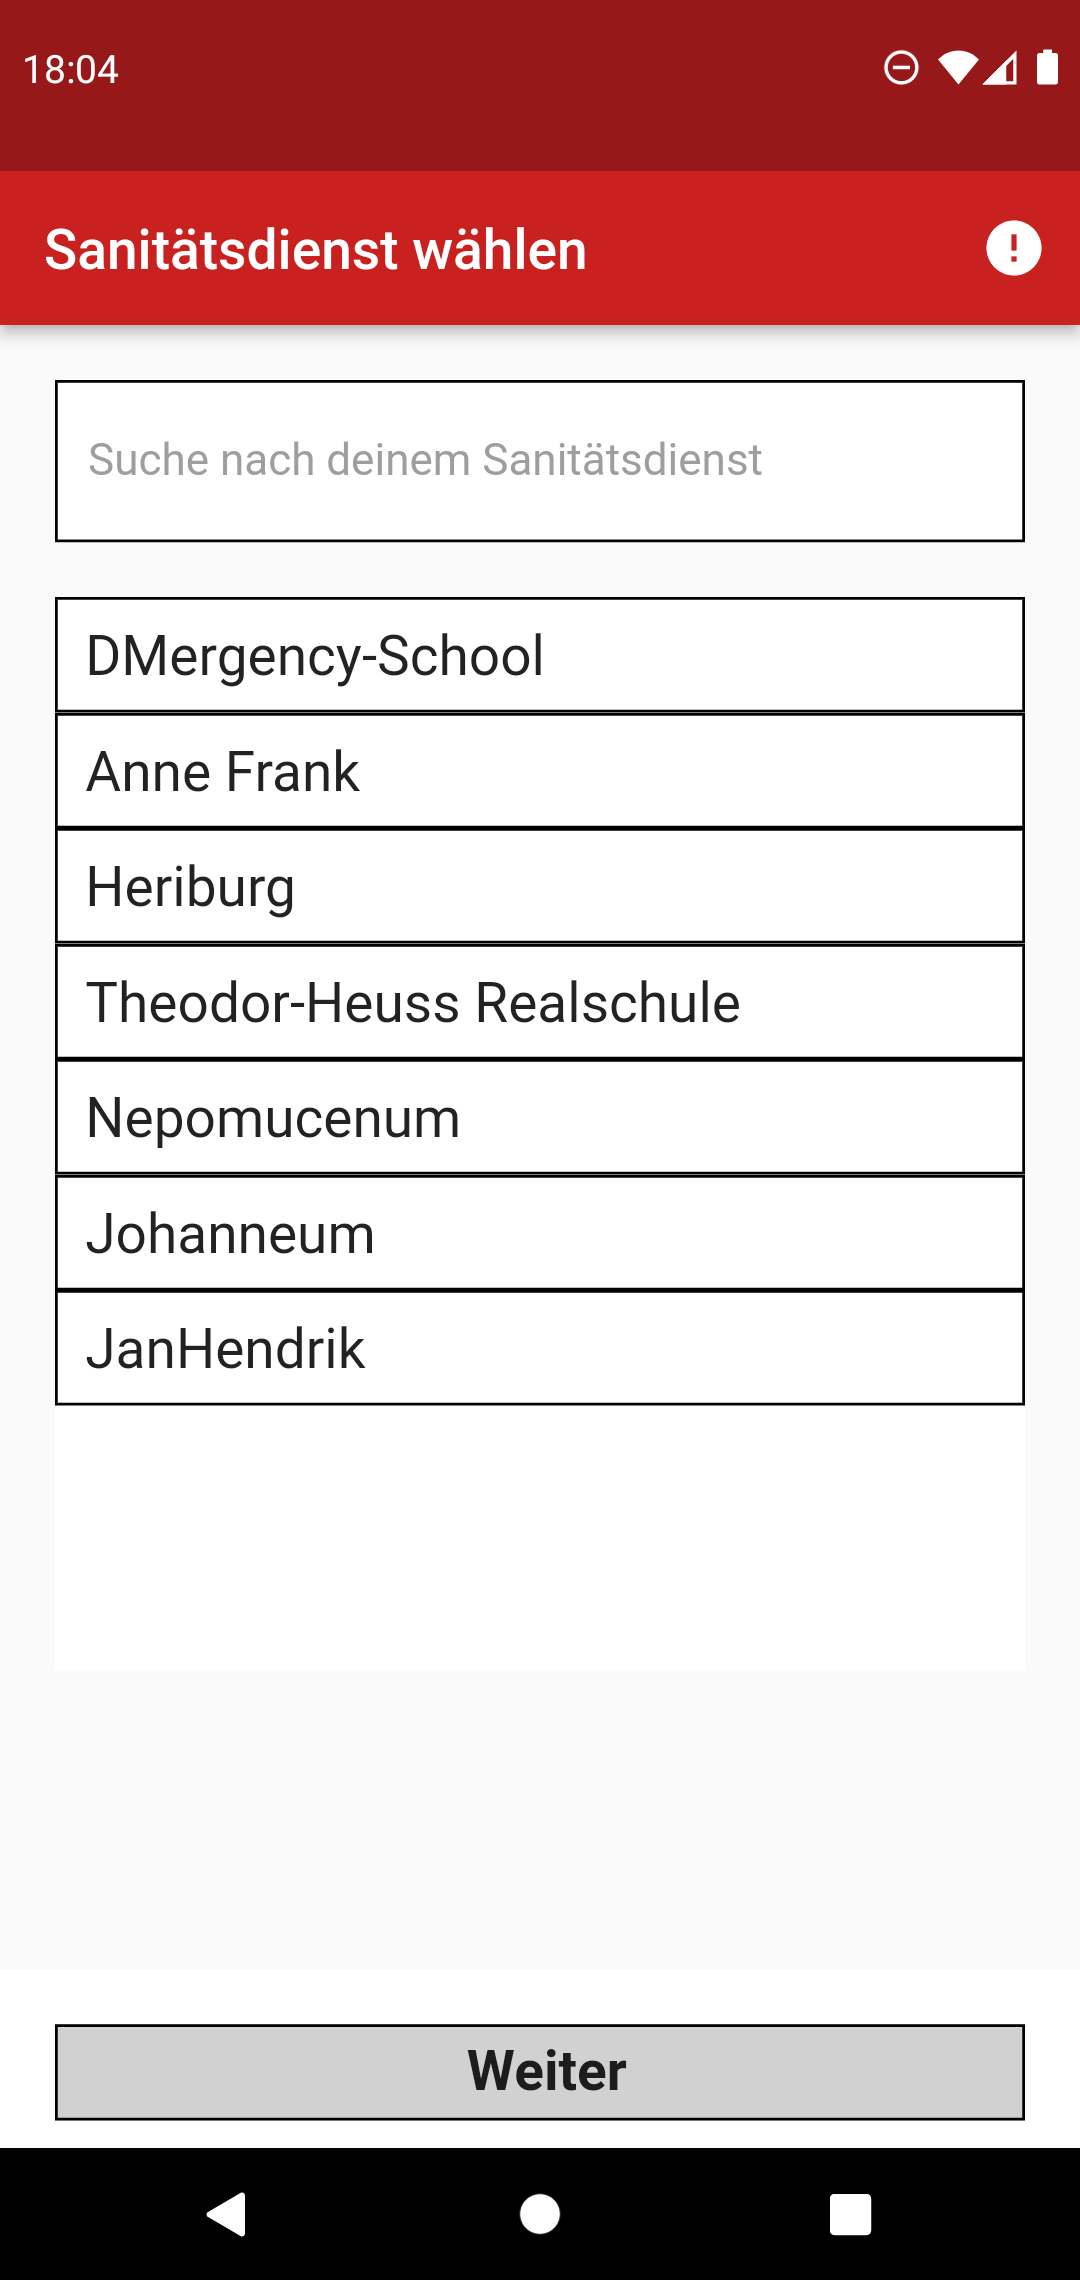
\includegraphics[width = 5cm]{images/SanitaetsdienstWahl.png}
        %    \end{center}
        %    \caption[Screenshot der Sanitätsdienst-Auswahl]{Beispielhafte Sanitätsdienst-
        %Auswahl}
        %\end{figure}
        
        \noindent Um vorher beschriebenes umzusetzen, muss beim Start der App zunächst überprüft werden, 
        ob bereits ein Nutzer eingeloggt ist oder nicht.
        \newline
        1. Es muss überprüft werden, ob schon ein Nutzer eingeloggt ist. In diesem 
        Fall soll keine Sanitätsdienstauswahl angezeigt werden, sondern
        die normale Nutzeroberfläche, für die entsprechende Rolle.
        \newline
        2. Ist bisher kein Nutzer eingeloggt, muss die Sanitätsdienstauswahl 
        angezeigt werden und die wählbaren Sanitätsdienste vom Server geladen 
        werden.
        \newline\\
        Nachdem der/die Sanitäter/-in dann seinen/ihren Sanitätsdienst ausgewählt hat,
        soll nun ein Login-View angezeigt werden, bei welchem der/die Nutzer/-in sich entscheiden 
        kann ob er/sie:
        \newline
        1. sich einloggen möchte.
        \newline
        2. sich neu registrieren möchte.
        \newline
        3. sein/ihr Passwort vergessen hat und dieses zurücksetzen möchte.
        \newline\\
        In der Nutzeroberfläche ist dies so umgesetzt, dass je ein Eingabefeld für
        die E-Mail-Adresse und das Passwort angegeben ist. Unter diesem sind dann je
        zwei Textfelder angelegt: \glqq Registrieren\grqq{} und \glqq Passwort vergessen\grqq{}, über
        welche dann auf die unterschiedlichen Views geleitet wird. Ganz unten in dem
        View erscheint dann erneut ein Button, welcher zum Anmelden genutzt werden 
        kann (Auch hier gibt es wieder die Unterscheidung wählbar/nicht wählbar).
        \\
        Im Code habe ich dies so umgesetzt, dass in einem View \glqq Validate\grqq{} ein 
        \glqq FutureBuilder\grqq{} zurückgegeben wird, der so lange einen LoadingIndicator angezeigt
        (Also einfach nur einen sich drehenden Kreis, der an einer Stelle eine Lücke hat)
        bis die \glqq future\grqq{} ausgeführt wurde. Die \glqq future\grqq{} ist eine Methode, welche 
        \texttt{async} (also asynchron) ist. In diesem Fall wird durch diese Methode die Rolle des/der Nutzer/-in 
        bestimmt. Hierfür werden zunächst die Login-Daten aus der Datenbank gelesen und 
        überprüft ob diese vorhanden sind. Danach wird kontrolliert, welche Nutzer/-innen Rolle in der 
        Datenbank steht und diese je nachdem passend für die API abgeändert (In der lokalen
        Datenbank ist 0 gespeichert, was für eine/-n Sanitäter/-in steht $\rightarrow$ 
        Abänderung zu 3, da ein/-e Sanitäter/-in bei der API eine 3 ist). Danach wird durch 
        eine Anfrage an den Server geprüft, ob der Nutzer noch existent ist, indem die 
        Sanitätsdienst-ID, die Nutzer-ID und die Rolle als \glqq query-Teil\grqq{} mitgegeben. Danach 
        wird abgeglichen, was die Antwort des Servers ist. Ist diese eine 0 wurde der Account 
        gelöscht und der/die Nutzer/-in wird ausgeloggt und auf die Sanitätsdienstauswahl 
        geleitet. Ist die Antwort eine 2, wird der/die Nutzer/-in auf den View der eigenen 
        Rolle weitergeleitet, kann jedoch keine Alarme versenden, da der Account 
        vorübergehend gesperrt ist. Bei diesen beiden Fällen wird jeweils ein AlertView 
        angezeigt, der darüber informiert, was \glqq falsch\grqq{} gelaufen ist (Zum Beispiel könnte
        hier dann angezeigt werden, dass der Account gesperrt ist).
        Dies ist implementiert worden, da die Administrator/-innen in der Lage sind Accounts zu löschen
        oder zu sperren, damit Nutzer/-innen, die die App ausnutzen gesperrt werden können.
        Im Falle einer 1 als Antwort ist alles normal und der/die Nutzer/-in wird auf den 
        passenden View für die jeweilige Rolle weitergeleitet. 

        \noindent Damit eine Anmeldung erfolgen kann, ist es notwendig einen bereits angelegten Account zu besitzen,
        den man auch in der App registrieren kann. Im Login-View die Eingabe der E-Mail-Adresse, 
        die mit dem Account verknüpft ist, sowie des zugehörigen Passwortes, um das Einloggen zu ermöglichen. 
        Die Account-Daten werden nach der Login-Bestätigung
        durch die App zum Server geschickt und überprüft, um dem/der Nutzer/-in
        im Anschluss eine Fehler-Meldung anzuzeigen oder sie/ihn auf die 
        Nutzeroberfläche weiterzuleiten.

        Um das Passwort zurücksetzen zu können, muss ein neuer \glqq View\grqq{} geöffnet werden, 
        in dem die persönliche E-Mail-Adresse eingegeben werden kann. Nachdem der/die Nutzer/-in
        diese bestätigt hat, erhält der/die Nutzer/-in eine E-Mail an die angegebene E-Mail-Adresse, die das
        Zurücksetzen des Passwortes ermöglicht.

        Das Registrier-Verfahren ist komplizierter. Nach dem Aufruf von \glqq Account erstellen\grqq{}
        Account erstellen ist es notwendig ein Passwort zur Registrierung anzugeben, dass
        durch die Leitung des Sanitätsdienstes festgelegt wurde. Dieses Passwort unterscheidet sich
        je nach Rolle, die zugeteilt werden soll. Das heißt: Nutzer/-in A soll die 
        Rolle Sanitäter/-in bekommen, so dass er/sie Passwort \glqq xyz\grqq angibt.
        Nutzer/-in B soll die Rolle Alarmierende/-r bekommen, also gibt die Person 
        Passwort \glqq abc\grqq an.
        \newline
        Nach der Verifizierung dieses Passworts erfolgt die weitere Registrierung der Rollen unterschiedlich: 
        \\\\
        1. Registrierung des/der Sanitäter/-in
        \newline Zunächst müssen Sanitäter/-innen ihren Vor- und Nachnamen zur 
        Identifizierung für die Sanitätsdienst-Leitung angeben. Außerdem muss eine 
        Stufe (bestehend aus drei beliebigen Zeichen) und ein Geschlecht angeben. 
        Diese Daten dienen der Sanitätsdienst-Leitung zur Identifizierung und Planung
        des Sanitätsdiensts. Dies Daten werden zum Beispiel für die Dienstplanung
        verwendet, da dieser möglichst divers sein sollte und nicht nur unerfahrene Sanitäter/-innen
        im Dienst sein sollen.\\ Danach muss der/die Nutzer/-in eine E-Mail-Adresse und
        ein Passwort angeben, um sich wieder anmelden zu können und den Nutzer im 
        System eindeutig zu identifizieren. Um sicher zu gehen, dass das gewünschte Passwort angegeben wurde,
        muss dieses zweimal eingegeben werden.
        Im Anschluss daran werden App-Berechtigungen abgefragt. Warum es diese
        gibt und weshalb diese Berechtigungen durch die App abgefragt werden, wird jetzt dargelegt.\\
        In den Betriebssystemen Android und iOS, gibt es zum einen Funktionen, die 
        ohne jegliche weitere Berechtigungen genutzt werden können (Dies 
        sind meist Funktionen, welche keine kritischen Nutzerdaten erfordern sondern
        nur zur App-Funktionalität beitragen. So zum Beispiel das Speichern von
        App-Daten). Jedoch stellen die beiden Herausgeber der jeweiligen Betriebssysteme 
        (Google und Apple) auch Funktionen zur Verfügung, welche Berechtigungen benötigen, 
        welche durch den Nutzer der App erlaubt werden müssen. Dies dient dem Datenschutz 
        der Nutzer/-innen der Betriebssysteme. Ich habe mich entschlossen einige 
        Berechtigungen abzufragen, damit ich den Nutzern einige Funktionen zur Verfügung 
        stellen kann. \\
        
        \noindent Bei Android-Geräten entschloss ich mich zu einer Abfrage, der Berechtigung, den 
        Nicht-Stören-Modus überschreiben zu können. Dies ermöglicht es der App jederzeit einen Alarmsound abspielen
        zu können, damit ein möglicherweise empfangener Alarm auch dann durch den Alarmsound bemerkt werden kann, wenn
        sich das Handy im \glqq Stumm\grqq{}- oder im \glqq Nicht-Stören\grqq{}-Modus befinden.
        Eine weitere Berechtigung auf Android-Geräten ist die Aufhebung der
        Batterie-Optimierung. Diese soll für die App deaktiviert werden, damit diese
        dauerhaft im Hintergrund läuft und die Alarme empfangen werden.\\ Auf 
        iOS-Geräten frage ich zum einen die Berechtigung ab, dass ich Mitteilungen senden darf, da 
        dies anders als bei Android eine Berechtigung erfordert, zum anderen frage 
        ich die Critical-Alert-Berechtigung ab, damit ich genauso wie bei 
        Android-Geräten den \glqq Stumm-\grqq{} und den \glqq Nicht-Stören-\grqq{}Modus überschreiben darf.
        %Überprüfen ob ich noch weitere Berechtigungen nutze
        %Warum gibt es die Berechtigungen, warum habe ich mich entschieden diese zu nutzen
        %\\
        \\\\ 2. Registrierung von Alarmierenden
        \\ Alarmierende müssen zunächst, ähnlich wie die Sanitäter/-innen, einen 
        Account-Namen festlegen. Dieser besteht jedoch nicht aus Vor- und Nachname 
        sondern nur aus einem generalisierten Namen. Hier können theoretisch auch 
        Account-Namen für feste Räume eingetragen werden, wie z.B. bei einem 
        Schulsanitätsdienst das Sekretariat. Danach muss, genauso, wie bei den 
        Sanitäter/-innen, eine E-Mail zur eindeutigen Identifikation eines Accounts
        angegeben werden, über welche auch das Passwort, welches im Anschluss 
        angegeben werden muss, zurückgesetzt werden kann. Das Passwort muss genauso
        wie bei den Sanitäter/-innen zweimal eingegeben werden, um die richtige 
        Eingabe von diesem sicherzustellen. Abschließend wird durch
        das Betätigen des \glqq Registrieren\grqq{}-Buttons die Registrierung abgeschlossen 
        werden und der/die Nutzer/-in wird auf das Nutzer-Interface weitergeleitet.


\subsubsection{Alarmauslösung}
    Das Auslösen des Alarmes soll, wie bereits erwähnt, möglichst einfach für die/den 
    Alarmierende/-n sein, da diese häufig Laien sind und sich in einer
    Alarmsituation bereits in einer Ausnahmesituation befinden und die App ein niederschwelliges 
    Angebot darstellen soll, sich auf einfache Art und Weise Hilfe zu holen.

     \noindent Um dies zu bewerkstelligen, sind auf dem Server Alarmorte vorgespeichert (Dies ist
     jedoch Teil des Servers und der Website, weshalb hier nicht weiter darauf eingegangen wird).
     Diese werden dann beim Aufruf des Views, auf dem der Alarm gesendet wird 
     heruntergeladen und im Anschluss angezeigt. Um diese auszuwählen, muss der/die 
     Nutzer/-in zunächst einen Ort-Typen aus einem Dropdown-Menü auswählen, welcher
     dann im Anschluss entscheidet, was als genauer Ort angegeben wird. Die genauen 
     Orte können entweder genau den gleichen Wert haben wie der Ort-Typ, oder eine 
     Auswahl an Objekten, oder eine Zeicheneingabe, welche entweder eine 
     Nummerneingabe oder eine Texteingabe sein kann. Diese werden entweder als 
     Dropdown-Menü, Eingabefeld oder als nicht abänderbarer Text angezeigt, je nachdem, was durch den Server definiert ist.
     Als ersten Schritt spezifiziert die alarmierende Person den Ort-Typen, danach 
     kann dieser dann den genauen Ort angeben. Im Anschluss kann der/die 
     Nutzer/-in eine Beschreibung des Geschehens verfassen, damit der/die 
     Sanitäter/-in sich bereits vor dem Eintreffen an der Einsatzstelle ein Bild von 
     der Lage machen kann, hierfür wird ein Eingabefeld angezeigt, in dem 
     der/die Nutzer/-in die Beschreibung angeben kann. Zuletzt kann der/die 
     Alarmierend/-e eine Priorität zwischen 1 und 5 festlegen, um die Dringlichkeit 
     deutlich zu machen. Hierbei ist 1 die niedrigste Priorität und 5 die höchste. Diese 
     Prioritätsauswahl ist durch RadioButtons (RadioButtons sind grafische Elemente zur Auswahl von genau einer 
     Option aus vielen) dargestellt.

    \noindent Der letzte Schritt, der dann noch ausgeführt werden muss, ist die 
    Betätigung des \glqq Alarm senden\grqq-Buttons, welcher dauerhaft sichtbar am 
    unteren Ende des Views angezeigt wird, um problemlos jederzeit alarmieren zu 
    können.

    Nach dem Senden des Alarms, das durch den Server geregelt wird, 
    nachdem von der App aus eine Request hierfür gestellt wurde, wird der 
    alarmierenden Person ein View angezeigt. Auf diesem kann rückverfolgt werden, 
    welche/-r Sanitäter/-in den Alarm entweder \glqq Empfangen\grqq{}, \glqq Abgelehnt\grqq{} 
    oder \glqq Bestätigt\grqq{} hat.
    Der Empfang des Alarms wird durch einen schwarzen Haken gekennzeichnet. Wird dieser bestätigt, erscheint ein
    grüner Haken, wird der Alarm abgelehnt, wird ein rotes X angezeigt. Erscheint ein Ladekreis, macht dieser deutlich,
    dass der Alarm noch nicht empfangen wurde.\\

    Folgend wird nun dargelegt, wie die Alarmierung implementiert wurde.
    Nach dem Drücken des Alarm-Buttons wird zunächst die Methode sendAlarm(BuildContext context)
    aufgerufen. Als Folge werden dann zuerst die Login-Daten aus der Datenbank gelesen, 
    um diese mit in die Alarmierungs-Request zu schreiben. Dies ist notwendig, um den Alarm nachverfolgen zu können.
    Im Anschluss darauf werden dann die 
    Beschreibung, die Priorität und der Alarmierungsort aus den jeweiligen Eingabefeldern 
    ausgelesen und ebenfalls in der Request angegeben. Danach wird die Request gesendet und 
    überprüft, ob es eine erfolgreiche Antwort des Servers gibt (also ob der http-Statuscode 
    200 ist, da dies signalisiert, dass eine valide Serverantwort zurückgegeben wurde) und ob die Antwort 
    eine gültige AlarmID enthält. Wenn diese Bedingungen zutreffen, 
    wird auf den bereits erwähnten Informations-View weitergeleitet, dem die AlarmID der 
    Serverantwort mitgegeben wird. Sollte eine der Bedingungen nicht erfüllt sein wird 
    ein AlertDialog angezeigt, der den/die Nutzer/-in über den Fehler informiert. Danach wird 
    bei beiden Fällen der View neu gebaut um die eingegeben Daten zurückzusetzen, damit ein neuer Alarm eingegeben 
    und gesendet werden kann.

\subsubsection{Alarmempfang}
    Wenn ein Alarm versendet werden kann, muss dieser logischerweise auch empfangen 
    werden können. Dies wird über ein Cloud-Messaging-System, Firebase 
    Cloud-Messaging, von Google, gelöst. Beim Empfangen des Alarms (also der 
    Nachricht von Firebase Cloud-Messaging), wird ein Alarm-Sound abgespielt, damit 
    der/die Sanitäter/-in diesen bemerkt. Im Anschluss an den ausgelösten Alarm-Sound werden die Alarm-Daten
    in die Datenbank geschrieben. Wenn der/die Sanitäter/-in die App nun öffnet, kann
    diese/-r den View \glqq Alarminformationen\grqq{} öffnen, auf welchem die empfangenen
    Alarme angezeigt werden. Klickt der/die Nutzer/-in jetzt auf den neuesten Alarm 
    werden die Alarminformationen hier erneut, jedoch detaillierter angezeigt.
    An dieser Stelle kann der/die Sanitäter/-in jetzt auch Rückmeldung auf den Alarm geben, in 
    dem er/sie diesen durch die jeweiligen Buttons ablehnt oder annimmt.
    Die Daten werden in der Reihenfolge Alarmierungszeitpunkt, Ort, Beschreibung, 
    Priorität angezeigt. Zum Einen dient dies der Information des 
    Sanitäters/ der Sanitäterin, zum Anderen soll so auch dem/der Sanitäter/-in 
    gezeigt werden, wann der Alarm gesendet, um einzuschätzen, wie dringlich ggf. zügig der Einsatz durchgeführt
    werden muss. Eine schlechte Internetverbindung, die ein verspätetes Eintreffen der Alarmierung zur Folge hat 
    oder ein schwerer Unfall, fordert sicherlich eine größere Eile als die Alarmierung zu einer Schürfwunde.
    Die Angabe des Ortes ist wichtig, da 
    der/die Sanitäter/-in dort möglichst zeitnah und an der richtigen Stelle eintreffen sollte. Erst dann 
    sind Beschreibung und Priorität wichtig, da dies nur Zusatzinformationen sind, 
    die der/die Sanitäter/-in so oder so am Einsatzort selbst erheben muss.

    \noindent Die Funktion der Alarm-Rückmeldung ist zum Einen zur Sicherstellung der
    Funktionsfähigkeit der App implementiert worden, zum Anderen soll so auch der 
    alarmierenden Person die Sicherheit gegeben werden, das Hilfe kommt, um sie in der 
    ihr vorliegenden Ausnahmesituation zu unterstützen beziehungsweise zu helfen.
    Die Alarmrückmeldung erfolgt über die Buttons am unteren Ende des Views. Zunächst
    sind die Buttons \glqq Bestätigen\grqq{} und \glqq Ablehnen\grqq{} gegeben. Im Anschluss wird
    entweder nur die Rückmeldung, die man selbst gegeben hat angezeigt, damit 
    der/die Sanitäter/-in dies überprüfen kann oder sollte man den Alarm bestätigt 
    haben und noch niemand anderes den Button \glqq Material holen\grqq{} betätigt hat, der eben genannte Button. 
    Dieser Button ist dafür gedacht, dass die Sanitäter/-innen sich untereinander absprechen können, wer das 
    Material holt. Wenn bereits von jemandem das Material 
    geholt wird, wird dies in einem weiteren Feld angezeigt und anstatt der Buttons 
    wird das Feedback für den Alarm angezeigt.

\subsubsection{Vertretungen}
    Um die Sanitäter/-innen zu alarmieren ist auf dem Server ein Dienstplan hinterlegt, 
    welcher bestimmt, wer an welchem Tag alarmiert wird. Jedoch kann es auch hier zu 
    Ausnahmesituationen kommen, in denen die eigentlich diensthabende Person nicht in 
    der Lage ist, den Dienst zu verrichten. Damit hier schnell eine Lösung gefunden 
    werden kann, ist es möglich, sich in der App zum Einen aus dem Dienst auszutragen.
    Zum anderen kann auch eine andere Person temporär für diesen Tag vertreten, wenn jemand  
    Bescheid gegeben hat, dass eine Person ihren Dienst nicht verrichten kann (Dies muss zurzeit noch parallel 
    zur App über ein anderes Medium stattfinden).  
    Dies wurde so umgesetzt, dass alle diensthabenden Personen
    innerhalb der App in einer Liste angezeigt werden. Der/die Nutzer/-in kann nun entweder 
    eine der diensthabenden Personen vertreten, in dem er/sie diese selbst auswählt und dann 
    auf \glqq Vertreten\grqq{} klickt, oder sich selbst austragen, in dem der/die Nutzer/-in auf den 
    \glqq Austragen \grqq Button klickt.

    Die Methode getCurrentDuties() lädt die aktuellen diensthabenden Sanitäter/-innen 
    herunter und fügt diese der angezeigten Liste hinzu. Dazu werden zunächst die 
    Sanitäter/-innen durch eine Request, in der die NutzerID und die SanitätsdienstID
    angegeben sind, heruntergeladen. Danach werden alle Einträge in diesem \glqq JSON-Array\grqq{} 
    durchgegangen und als DienstModel der Liste hinzugefügt. Dabei ist das Attribut 
    isUser dafür da, dass der/die Nutzer/-in in der App hervorgehoben wird, wenn er/sie 
    selbst im Dienst ist. Danach wird noch überprüft, ob der/die Nutzer/-in die 
    Berechtigungen hat, den Dienst einzusehen und zu vertreten / sich auszutragen. Ebenso wird geprüft, ob
    ob die auszuführende Aktion für den Button das Austragen oder das Vertreten ist, 
    je nachdem ob die Person selbst gerade im Dienst ist oder nicht.

\subsubsection{News \& Notfallnummern}
    Um dem Sanitätsdienst eine gute Kommunikation zu ermöglichen, wurde zusätzlich ein 
    News-Feature implementiert. Hier ist zurzeit nur das Anzeigen der News, die auf 
    dem Server gespeichert sind, möglich und nicht das Erstellen von neuen News. Die News 
    werden genutzt, um die interne Kommunikation des Sanitätsdienstes zu vereinfachen.

    Um der alarmierenden Person zusätzliche Sicherheit zu geben ist außerdem ein View 
    implementiert worden, auf dem die wichtigsten Notfallnummern aufgelistet sind,
    damit diese die entsprechende Nummer im Notfall durch anklicken der Nummer anrufen 
    kann und sich nicht zwingend an diese erinnern muss. Es wird hier nach dem Klicken 
    ein AlertView angezeigt, bei der/die Nutzer/-in entscheiden kann, ob er/sie tatsächlich die 
    angeklickte Notfallnummer wählen möchte, falls dieser/diese sich verklickt haben sollte.
    
\subsubsection{Berechtigungen \& Fehler}
    Um der Sanitätsdienst-Leitung möglichst viel Kontrolle zu geben, was von den 
    Sanitäter/-innen gesehen und getan werden kann, gibt es einige Berechtigungen, die 
    auf dem Server gespeichert sind. Die einfachste und zugleich schwerwiegendste 
    Berechtigung ist das Sperren von einem Account. Diese Berechtigung ist dafür 
    gedacht, dass, sollte ein/e Sanitäter/-in oder ein/-e Alarmierende/-r die App
    fälschlicherweise nutzen, dieser gesperrt werden kann.

    Es gibt jedoch auch weniger drastische Mittel, mit denen die Nutzer/-innen in dem was sie tun,
    eingeschränkt werden können. Zum einen kann die Berechtigung 
    mit hohen Prioritäten zu alarmieren(z.B. wenn die Person immer 
    mit Priorität 5 alarmiert obwohl dies nicht notwendig wäre) entzogen werden.  
    Die Berechtigung zu alarmieren kann ebenfalls entzogen werden, wenn die Alarmierung in der 
    Form ausgenutzt wird, dass die Sanitäter/-innen in hohem Maße unnötiger Weise alarmiert werden.

    Außerhalb der Alarmierung gibt es auch Berechtigungen bei dem Vertretungssystem. 
    Hier gibt es die Möglichkeit den Sanitäter/-innen die Berechtigung zu entziehen 
    zu vertreten oder sich aus dem Dienst auszutragen. Ein Anwendungsfall hierfür wäre 
    zum Beispiel, dass sich Sanitäter/-innen ständig ohne ersichtlichen Grund aus dem Dienst 
    austragen oder andere Sanitäter/-innen ohne Absprache streichen, um selbst Dienst übernehmen zu können.

    Die letzte Möglichkeit Nutzer/-innen einzuschränken ist es die Berechtigung zu entziehen, 
    eigene empfangenen Alarme einzusehen. Ein Grund hierfür könnte gegeben sein, wenn Alarmdaten an 
    unbefugte Personen weitergegeben wurden und dies nun 
    verhindert werden soll. Die Berechtigungen werden beim Server angefragt und dann je 
    nach View umgesetzt. Der JSON-Array, der vom Server geladen wird, kann dann 
    Folgendermaßen aussehen: [101, 102, 201, 202, 301, 302, 303, 304, 707, 708].

    Damit der Nutzer nicht vergeblich z.B.  auf einen Sanitäter wartet, wenn eine Fehler auftritt,  
    wird diesem ein AlertView angezeigt. Somit hat er die Möglichkeit darauf zu reagieren.